\question{考虑载电流\nota{I}的无穷长细直导线,利用毕奥-萨伐尔定律,通过直接积分求磁感应强度。}

    \begin{figure}[htbp]
        \centering
        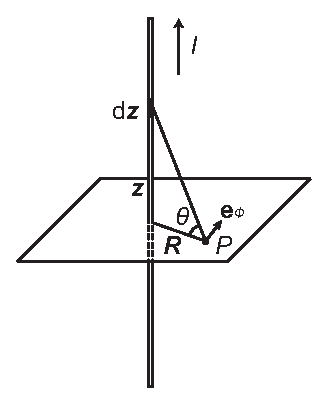
\includegraphics{img/3.1/导线.eps}
        \caption{无穷长直导线}
        \label{3.1_fig:导线}
    \end{figure}
    
    如图\ref{3.1_fig:导线},取导线沿\nota{z}轴,设\nota{P}点到导线的垂直距离为\nota{R},电流元\nota{I\d z}到\nota{P}点的矢径为\nota{\r},有毕奥-萨伐尔定律
    \begin{equation}
        B(P) = \frac{\mu I}{4\pi}\int_{-\infty}^{+\infty}
        \frac{\d \z\times \r}{r^3}\label{3.1_1}
    \end{equation}
    如图\ref{3.1_fig:导线},设\nota{\r}与\nota{\bm R}的夹角为\nota{\theta},注意到几何关系
    \begin{equation}
        |\d \z| = R \frac{1}{\cos^2\theta}\d \theta\label{3.1_2}
    \end{equation}
    \begin{equation}
        \d \z \times \r = |\d \z| r \cos \theta \danwei{\phi}\label{3.1_3}
    \end{equation}
    \begin{equation}
        r = \frac{R}{\cos\theta}\label{3.1_4}
    \end{equation}
    由(\ref{3.1_1})(\ref{3.1_2})(\ref{3.1_3})(\ref{3.1_4})得
    \begin{equation}
        B(P) = \frac{\mu I\danwei{\phi}}{4\pi R}\int_{-\pit}^{+\pit}\cos\theta\d \theta = \frac{\mu I\danwei{\phi}}{2\pi R}\label{3.1_5}
    \end{equation}

\question{求下面两个矢势对应的磁感应强度:}

    \subquestion{\nota{A_x = A_y = 0,\quad A_z = -y B_0}(其中\nota{\bz}为常数);}
    
    根据矢势的定义,可以直接写出
    \begin{equation}
        \b = \nabla \times \a = \dreieinss \ep \partial_i A_j \bm{e}_k = -\bz \bm{e}_x
    \end{equation}
    
    \subquestion{\nota{A_x = A_z = 0,\quad A_y = x B_0}(其中\nota{\bz}为常数)。}
    
    \begin{equation}
        \b = \nabla \times \a = \dreieinss \ep \partial_i A_j \bm{e}_k = \bz \bm{e}_z
    \end{equation}
